\documentclass[10pt,varwidth]{standalone}
% \documentclass[12pt]{article}
% 1.必须添加varwidth选项,不然就会报错
% \PassOptionsToPackage{quiet}{fontspec}
% \usepackage{ctex}
\usepackage{geometry}
\geometry{a2paper,left=1in,right=1in,top=1in,bottom=1in}
\usepackage{pgfplots}
\usepackage{pgfplotstable}
\pgfplotsset{compat=1.16}
% 2.引用的tikz库
\usetikzlibrary{matrix,chains,trees,scopes,decorations}
\usetikzlibrary{arrows.meta,automata,positioning,shadows,3d}
\usetikzlibrary {decorations.pathmorphing}
\usetikzlibrary {backgrounds,mindmap,shadows}
\usetikzlibrary {patterns, quotes}
\usetikzlibrary {graphs,fadings}
\usetikzlibrary {arrows,shapes.geometric}
\usepgflibrary {shadings}
\newcommand{\Vdots}[2]{%
    \begin{scope}
        \node[circle, fill, inner sep=1pt] (A) at (#1, #2+0.2) {};
        \node[circle, fill, inner sep=1pt] (B) at (#1, #2) {};
        \node[circle, fill, inner sep=1pt] (C) at (#1, #2-0.2) {};
    \end{scope}
}

\tikzset{
    >={Latex[length=6mm, width=2mm]}
}




\begin{document}
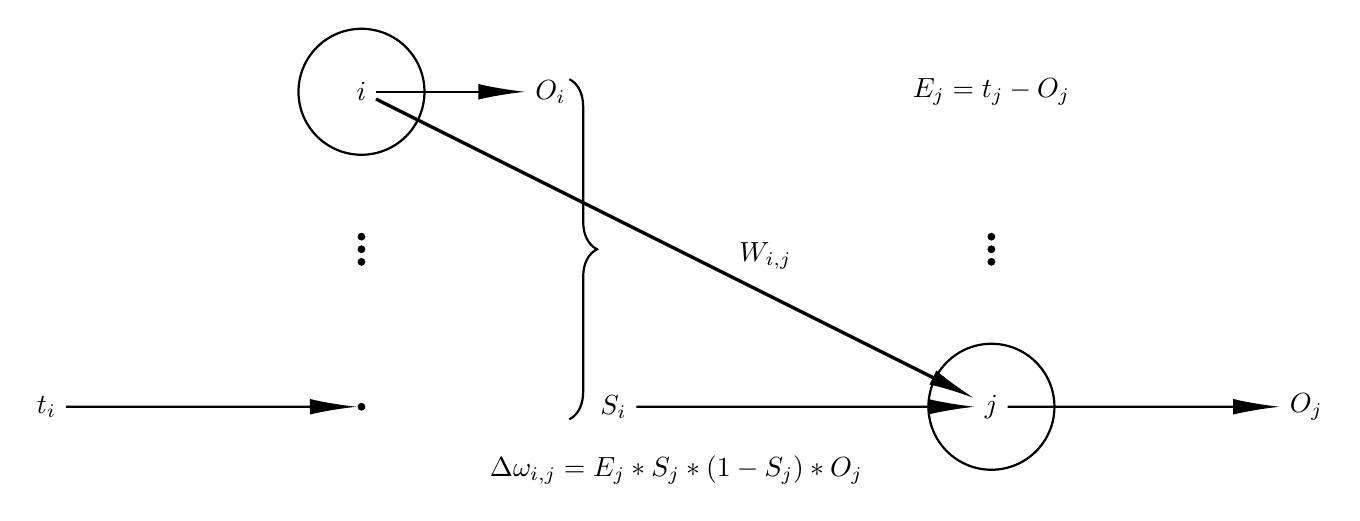
\begin{tikzpicture}[scale=.8]
    % 1.节点标注
    \node(A13) at (0, -5) {$t_i$};
    \node(A21) at (5, 0) {$i$};
    \node[circle, fill, inner sep=1pt] (A23) at (5, -5) {};
    \node(A31) at (8, 0) {$O_i$};
    \node(A43) at (9, -5) {$S_i$};
    \node(A51) at (15, 0) {$E_j = t_j-O_j$};
    \node(A53) at (15, -5) {$j$};
    \node(A63) at (20, -5) {$O_j$};


    % 2.基本框架
    \draw[->, thick] (A13) -- (A23);

    \draw[thick] (A21) circle(1);
    \draw[->, very thick] (A21) -- node[pos=.65, above=5pt]{$W_{i, j}$}(A53);
    \draw[->, thick] (A21) -- (A31);
    \Vdots{5}{-2.5}
    \draw[thick,decorate,decoration={brace, amplitude=10pt}] (8.3, 0.2) -- (8.3, -5.2);
    \draw[->, thick] (A43) -- (A53);

    \draw[thick] (A53) circle(1);
    \Vdots{15}{-2.5}
    \draw[->,thick] (A53) -- (A63);

    % 图注
    \node at (10, -6) {$\Delta \omega_{i, j} = E_j*S_j*(1-S_j)*O_j$}; 



















\end{tikzpicture}
\end{document}